\documentclass{juliacon}
\setcounter{page}{1}

\begin{document}

% **************GENERATED FILE, DO NOT EDIT**************

\title{Explaining Black-Box Models through Counterfactuals}

\author[1]{Patrick Altmeyer}
\author[1]{Arie van Deursen}
\author[1]{Cynthia C. S. Liem}
\affil[1]{Delft University of Technology}

\keywords{Julia, Explainable Artificial Intelligence, Counterfactual Explanations, Algorithmic Recourse}

\hypersetup{
pdftitle = {Explaining Black-Box Models through Counterfactuals},
pdfsubject = {JuliaCon 2022 Proceedings},
pdfauthor = {Patrick Altmeyer, Arie van Deursen, Cynthia C. S. Liem},
pdfkeywords = {Julia, Explainable Artificial Intelligence, Counterfactual Explanations, Algorithmic Recourse},
}



\maketitle

\begin{abstract}

Machine learning models like deep neural networks have become so complex and opaque over recent years that they are generally considered as black boxes. Nonetheless such models often play a key role in modern automated decision-making systems. Counterfactual explanations can help programmers make sense of the systems they build: they explain how inputs into a system need to change for it to produce different decisions. Explanations that involve realistic and actionable changes can be used for the purpose of algorithmic recourse: they offer individuals subject to algorithms a way to turn a negative decision into positive one. In this article we discuss the usefulness of counterfactual explanations for interpretable machine learning and demonstrate its implementation in Julia using the \verb|CounterfactualExplanations| package.

\end{abstract}

\hypertarget{sec-intro}{%
\section{Introduction}\label{sec-intro}}

Advances in technology have typically gone hand in hand with an
outsourcing of labour from humans to machines: the printing press
succeeded human scribes centuries ago, ATMs replaced bank tellers
decades ago and today robots are swarming factory floors. While these
transitions involved a subsitution of manual or repetitive tasks, recent
advances in computing and artificial intelligence (AI) have accelerated
a new type of transformation: from human to data-driven decision-making.
Today, it is more likely than not that your digital loan or employment
application will be handled by an algorithm, at least in the first
instance. This can in theory be beneficial to you: automation typically
leads to increased efficiency and has the potential to remove human bias
and error. In reality though, state-of-the-art algorithms are often
instable (\cite{goodfellow2014explaining}), encode existing biases
(\cite{buolamwini2018gender}) and learn representations that are
surprising or even counter-intuitive form a human perspective
(\textbf{REFERENES?} \cite{}).

This is made more problematic by the fact that many modern machine
learning algorithms tend to be so complex and underspecified in the
data, that they are essentially black boxes. While this is a known
issue, such models are still used to guide decision-making and research
in industry as well as academia. At the time of writing, the largest
artificial neural networks are made up of several hundreds of billion
neurons. In the context of high-stake decision-making systems, black-box
models create undesirable dynamics: the human operators in charge of the
system have to rely on it blindy, while those indviduals subject to it
generally have no way to challenge an outcome. If your digital loan or
employment application gets rejected, for example, that is typically the
end of the story.

\begin{quote}
``You cannot appeal to (algorithms). They do not listen. Nor do they
bend.''

--- Cathy O'Neil in
\href{https://en.wikipedia.org/wiki/Weapons_of_Math_Destruction}{\emph{Weapons
of Math Destruction}}, 2016
\end{quote}

While the inappropriate abuse of such technologies is arguably the
biggest issue, we should also be concerned about missed opportunities.
The lack of trustworthiness in machine learning prevents it from being
adopted in other fields of research, which might actually benefit from
its adoption. Economics and financial markets, for example, are full of
complexities and non-linearities that machine learning algorithms are
well-equipped to model. But financial practitioners and policy makers
are understandably wary of using tools they cannot fully understand
(\cite{oecd2021artificial},\cite{hansen2020virtue}).

In light of all this, a quickly growing body of literature on
explainable artificial intelligence has emerged. Counterfactual
explanations (CE) and algorithmic recourse (AR) fall into this broader
category. Counterfactual explanations can help programmers make sense of
the systems they build: they explain how inputs into a system need to
change for it to produce different decisions. Explanations that involve
realistic and actionable changes can be used for the purpose of
algorithmic recourse (AR): they offer individuals subject to algorithms
a way to turn a negative decision into positive one. Through the
\texttt{CounterfactualExplanations} package we aim to contribute a
scalable and verstile implementation of CE and AR to the Julia
community. The remainder of this article is structured as follows:
Section~\ref{sec-related} presents related work on explainable AI,
Section~\ref{sec-method} provides a brief overview of the methodological
framework, Section~\ref{sec-use} presents the package functionality and
Section~\ref{sec-conclude} concludes.

\hypertarget{sec-related}{%
\section{Related work on explainable ML}\label{sec-related}}

\hypertarget{sec-method}{%
\section{Methodological background}\label{sec-method}}

Counterfactual search happens in the feature space: we are interested in
understanding how we need to change individual attributes in order to
change the model output to a desired value or label
(\cite{molnar2020interpretable}). Typically the underlying methodology
is presented in the context of binary classification:
\(M: \mathcal{X} \mapsto y\) where and \(y\in\{0,1\}\). Let \(t=1\) be
the target class and let \(\overline{x}\) denote the factual feature
vector of some individual outside of the target class, so
\(\overline{y}=M(\overline{x})=0\). We follow this convention here,
though it should be noted that the ideas presented here also carry over
to multi-class problems and regression (\cite{molnar2020interpretable}).

\hypertarget{generic-framework}{%
\subsection{Generic framework}\label{generic-framework}}

Then the counterfactual search objective originally proposed by
\cite{wachter2017counterfactual} is as follows

\begin{equation}\protect\hypertarget{eq-obj}{}{
\min_{\underline{x} \in \mathcal{X}} h(\underline{x}) \ \ \ \mbox{s. t.} \ \ \ M(\underline{x}) = t
}\label{eq-obj}\end{equation}

where \(h(\cdot)\) quantifies how complex or costly it is to go from the
factual \(\overline{x}\) to the counterfactual \(\underline{x}\). To
simplify things we can restate this constrained objective
(Equation~\ref{eq-obj}) as the following unconstrained and
differentiable problem:

\begin{equation}\protect\hypertarget{eq-solution}{}{
\underline{x} = \arg \min_{\underline{x}}  \ell(M(\underline{x}),t) + \lambda h(\underline{x})
}\label{eq-solution}\end{equation}

Here \(\ell\) denotes some loss function targeting the deviation between
the target label and the predicted label and \(\lambda\) governs the
stength of the complexity penalty. Provided we have gradient access for
the black-box model \(M\) the solution to this problem
(Equation~\ref{eq-solution}) can be found through gradient descent. This
generic framework lays the foundation for most state-of-the-art
approaches to counterfactual search and is also used as the baseline
approach - \texttt{GenericGenerator} - in our package. The
hyperparameter \(\lambda\) is typically tuned through grid search.
Conventional choices for \(\ell\) include margin-based losses like
cross-entropy loss and hinge loss. It is worth pointing out that the
loss function is typically computed with respect to logits rather than
predicted probabilities, a convetion that we have chosen to
follow.\footnote{While the rationale for this convention is not entirely
  obvious, implementations of loss functions with respect to logits are
  often numerically more stable. For example, the
  \texttt{logitbinarycrossentropy(ŷ,\ y)} implementation in
  \texttt{Flux.Losses} (used here) is more stable than the
  mathematically equivalent \texttt{binarycrossentropy(ŷ,\ y)}.}

Numerous - and in some cases competing - extensions to this simple
approach have been developed since counterfactual explanations were
first proposed in 2017 (see \cite{verma2020counterfactual} and
\cite{karimi2020survey} for surveys). The various approaches largely
differ in how they define the complexity penalty. In
\cite{wachter2017counterfactual}, for example, \(h(\cdot)\) is defined
in terms of the Manhattan distance between factual and counterfactual
feature values. While this is an intuitive choice, it is too simple to
address many of the desirable properties of effective counterfactual
explanations that have been set out. These desiderata include:
\textbf{closeness} - the average distance between factual and
counterfactual features should be small
(\cite{wachter2017counterfactual}); \textbf{actionability} - the
proposed feature perturbation should actually be actionable
(\cite{ustun2019actionable}, \cite{poyiadzi2020face});
\textbf{plausibility} - the counterfactual explanation should be
plausible to a human (\cite{joshi2019towards}); \textbf{unambiguity} - a
human should have no trouble assigning a label to the counterfactual
(\cite{schut2021generating}); \textbf{sparsity} - the counterfactual
explanation should involve as few individual feature changes as possible
(\cite{schut2021generating}); \textbf{robustness} - the counterfactual
explanation should be robust to domain and model shifts
(\cite{upadhyay2021towards}); \textbf{diversity} - ideally multiple
diverse counterfactual explanations should be provided
(\cite{mothilal2020explaining}); and \textbf{causality} - counterfactual
explanations reflect the structual causal model underlying the data
generating process
(\cite{karimi2020algorithmic},\cite{karimi2021algorithmic}).

\hypertarget{counterfactuals-for-bayesian-models}{%
\subsection{Counterfactuals for Bayesian
models}\label{counterfactuals-for-bayesian-models}}

For what follows it is worth elaborating on the approach proposed in
\cite{schut2021generating}. The authors demonstrate that many of the
abovementioned desiderata can be addressed very easily, if the
classifier \(M\) is Bayesian. In particular, they show that close,
realistic, sparse and unambigous counterfactuals can be generated by
implicitly minimizing the classifier's predictive uncertainty through a
greedy counterfactual search. Formally, they define \(h(\cdot)\) as the
predictive entropy of the classifier, which captures both
\textbf{epistemic} and \textbf{aleatoric} uncertainty: the former is
high on points far away from the training data while the latter is high
in regions of the input space that are inherently noisy. Both are
regions we want to steer clear off in our counterfactual search and
hence predictive entropy is an intuitive choice for a complexity
penalty. The authors further point out that any solution that minimizes
cross-entropy loss (Equation~\ref{eq-solution}) also minimizes
predictive entropy:
\(\arg \min _{\underline{x}} \ell(M(\underline{x}),t) \in \arg \min _{\underline{x}} h(\underline{x})\).
Let \(\mathcal{\widetilde{M}}\) denote the class of binary classifiers
that incorporate predictive uncertainty, then the previous observation
implies that the optimal solution to counterfactual search
(Equation~\ref{eq-solution}) can be restated as follows:

\begin{equation}\protect\hypertarget{eq-solution-bayes}{}{
\underline{x} = \arg \min_{\underline{x}}  \ell(M(\underline{x}),t) \ \ , \ \  \forall M\in\mathcal{\widetilde{M}}
}\label{eq-solution-bayes}\end{equation}

We can drop the complexity penalty altogether and still generate
effective counterfactual explanations. As we will see below, even a fast
and greedy counterfactual search proposed in \cite{schut2021generating}
yields good results in this setting. The approach has been implemented
as \texttt{GreedyGenerator} in our package and should only be used with
classifiers of type \(\mathcal{\widetilde{M}}\). It is worth noting that
the findings in \cite{schut2021generating} are not mutually exclusive of
many of the other methodologies that have been put foward. On the
contrary, we believe that they are complementary: the generic
counterfactual search proposed in \cite{wachter2017counterfactual}, for
example, can be shown to produce more plausible counterfactuals in the
Bayesian setting. Similarly, there is no obvious reason why recent work
on diversity (\cite{mothilal2020explaining}), robustness
(\cite{upadhyay2021towards}) and causality
(\cite{karimi2020algorithmic},\cite{karimi2021algorithmic}) could not be
complemented by the findings in \cite{schut2021generating}. For this
reason we are highlighting \cite{schut2021generating} here and have
prioritized it in the development of
\texttt{CounterfactualExplanations}. While there is no free lunch and
\(M\in\mathcal{\widetilde{M}}\) may seem like a hard constraint, recent
advances in probabilistic machine learning have shown that the
computational cost involved in Bayesian model averaging is lower than we
may have thought (\cite{gal2016dropout},
\cite{lakshminarayanan2016simple}, \cite{daxberger2021laplace},
\cite{murphy2022probabilistic}).

\hypertarget{sec-use}{%
\section{\texorpdfstring{Using
\texttt{CounterfactualExplanations}}{Using CounterfactualExplanations}}\label{sec-use}}

The package is built around two modules that are designed to be as
scalable as possible through multiple dispatch: 1) \texttt{Models} is
concerned with making any arbitrary model compatible with the package;
2) \texttt{Generators} is used to implement arbitrary counterfactual
search algorithms.\footnote{We have made an effort to keep the code base
  a flexible and scalable as possible, but camodelot guarantee at this
  point that really any counterfactual generator can be implemented
  without further adaptation.} The core function of the package
\texttt{generate\_counterfactual} uses an instance of type
\texttt{T\ \textless{}:\ FittedModel} produced by the \texttt{Models}
module (Figure~\ref{fig-models}) and an instance of type
\texttt{T\ \textless{}:\ Generator} produced by the \texttt{Generators}
module (Figure~\ref{fig-generators}). Relating this back the methodology
outlined in Section~\ref{sec-method}, the former instance corresponds to
the model \(M\) while the latter defines the rules for the
counterfactual search (Equation~\ref{eq-solution} and
Equation~\ref{eq-solution-bayes}). In the following we will demonstrate
how to use and extend the package architecture through a few examples.

\begin{figure}

{\centering 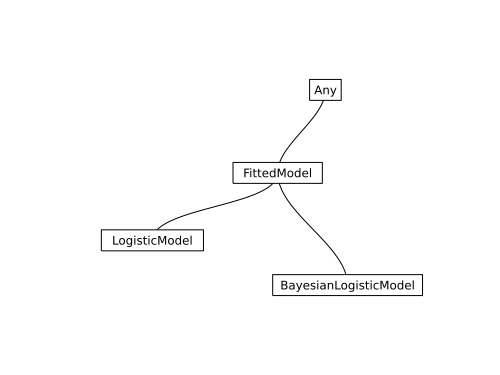
\includegraphics[width=3.33333in,height=2.5in]{www/models.png}

}

\caption{\label{fig-models}Schematic overview of the
\texttt{FittedModel} base type and its descendants.}

\end{figure}

\begin{figure}

{\centering 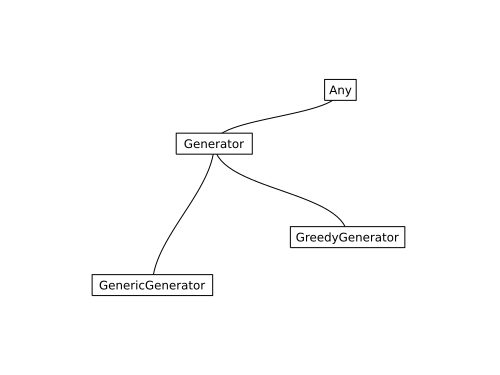
\includegraphics[width=3.33333in,height=2.5in]{www/generators.png}

}

\caption{\label{fig-generators}Schematic overview of the
\texttt{Generator} base type and its descendants.}

\end{figure}

\hypertarget{sec-start}{%
\subsection{Getting started}\label{sec-start}}

The code below provides a complete example demonstrating how the
framework presented in Section~\ref{sec-method} can be implemeted in
Julia using the \texttt{CounterfactualExplantions} package: using a
synthetic data set with linearly separable samples we firstly define our
model and then generate a counterfactual for a randomly selected sample.
Figure~\ref{fig-binary} shows the resulting counterfactual path in the
two-dimensional feature space: features go through iterative
perturbations until the desired confidence level is reached as
illustrated by the contour in the background, which indicates the
classifier's predicted probability that the label is equal to 1.

It may help to go through the relevants parts of the code in some more
detail starting from the part involving the model. For illustrative
purposes the \texttt{Models} module ships with a constructor for a
logistic regression model:
\texttt{LogisticModel(W::Matrix,b::AbstractArray)\ \textless{}:\ FittedModel}.
This constructors does not fit the regression model, but rather takes
its underlying parameters as given. In other words, it is generally
assumed that the user has already estimated a model. Based on the
provided estimates two functions are already implemented that compute
logits and probabilities for the model, respectively. Below we will see
how users can use multiple dispatch to extend these functions for use
with arbitrary models. For now it is enough to note that those methods
define how the model makes its predictions \(M(x)\) and hence they form
an integral part of the counterfactual search.

With the model \(M\) defined in the code below we go on to set up the
counterfactual search as follows: 1) choose a random sample
\texttt{x\_factual}; 2) compute its factual label \texttt{y\_factual} as
predicted by the model (\(M(\overline{x})=0\)); and 3) specify the other
class as our \texttt{target} label (\(t=1\)) along with a desired level
of \texttt{confidence} in the final prediction \(M(\underline{x})=t\).

The last two lines of the code below define the counterfactual generator
and finally run the counterfactual search. The first three fields of the
\texttt{GenericGenerator} are reserved for hyperparameters governing the
strength of the complexity penalty, the step size for gradient descent
and the tolerance for convergence. The fourth field accepts a
\texttt{Symbol} defining the type of loss function \(\ell\) to be used.
Since we are dealing with a binary classification problem logit binary
cross-entropy is an appropriate choice.\footnote{As mentioned earlier,
  the loss function is computed with respect to logits and hence it is
  important to use logit binary cross-entropy loss as opposed to just
  binary cross-entropy.} The fifth and last field can be used to define
mutability constraints for the features.

\begin{lstlisting}[language = Julia]
# Data:
using CounterfactualExplanations, Random
Random.seed!(1234)
N = 100 # number of data points
using CounterfactualExplanations.Data
x, y = toy_data_linear(N) 

# Model:
using CounterfactualExplanations.Models 
w = [1.0 1.0]# true coefficients
b = 0
M = LogisticModel(w, [b])

# Setup:
x_factual = x[rand(1:length(x))]
y_factual = round(probs(M, x_factual)[1])
target = ifelse(y_factual==1.0,0.0,1.0) 
confidence = 0.75 

# Counterfactual search:
generator = GenericGenerator(
    0.1,0.1,1e-5,:logitbinarycrossentropy,nothing)
counterfactual = generate_counterfactual(
    generator, x_factual, M, target, confidence)
\end{lstlisting}

\begin{figure}

{\centering 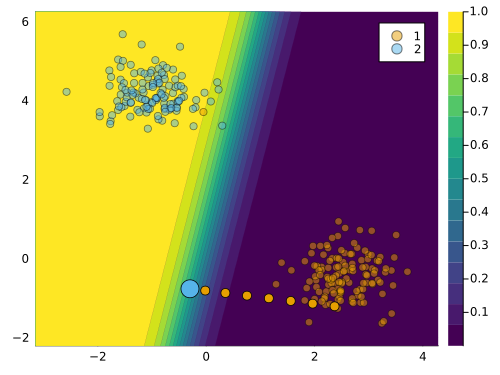
\includegraphics[width=3.33333in,height=2.5in]{www/ce_binary.png}

}

\caption{\label{fig-binary}Counterfactual path using generic
counterfactual generator for conventional binary classifier.}

\end{figure}

In this simple example the generic generator produces an effective
counterfactual: the decision boundary is crossed (i.e.~the
counterfactual explanation is valid) and upon visual inspection the
counterfactual seems plausible (Figure~\ref{fig-binary}). Still, the
example also illustrates that things may well go wrong: since the
underlying model produces high-confidence predictions in regions free of
any data, it is easy to think of scenarios that involve valid but
unrealistic or ambiguous counterfactuals. Consider, for example, the
scenario illustrated in Figure~\ref{fig-binary-wrong}, which involves
the same logisitic classifier albeit massively overfitted. In this case
generic search may yield an unrealistic counterfactual that is well into
the yellow region and yet far away from all other samples (red marker)
or an ambiguous counterfactual near the decision boundary (black
marker).

\begin{figure}

{\centering 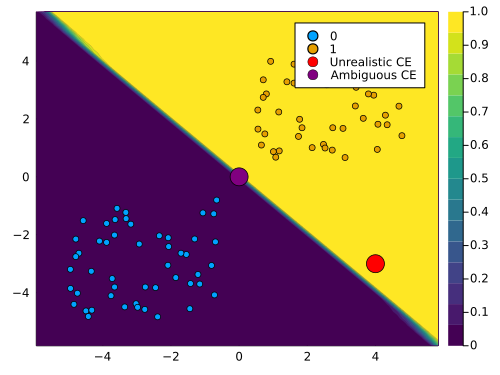
\includegraphics[width=3.33333in,height=2.5in]{www/binary_wrong.png}

}

\caption{\label{fig-binary-wrong}Unrealistic and ambiguous
counterfactuals that may be produced by generic counterfactual search
for an overfitted conventional binary classifier.}

\end{figure}

Among the different approaches that have recently been put forward to
deal with such issues is the greedy generator for Bayesian models
proposed by \cite{schut2021generating}. For reasons discussed in
Section~\ref{sec-method}, we have chosen to prioritize this approach in
the development of \texttt{CounterfactualExplanations}. The code below
shows how this approach can be implemented.
Figure~\ref{fig-binary-laplace} shows the resulting counterfactual path
through the feature space along with the predicted probabilities from
the Bayesian classifier.

Once again it is worth dwelling on the code for a moment. We have used
the same synthetic toy data as before, but this time we use assume that
we have fit a Bayesian logistic regression model through Laplace
approximation. This approximation uses the fact the second-order Taylor
expansion of the logit binary cross-entropy function evaluated at the
maximum-a-posteriori (MAP) estimate amounts to a multivariate Gaussian
distribution (\cite{murphy2022probabilistic}).\footnote{See also this
  \href{https://www.paltmeyer.com/blog/posts/effortsless-bayesian-dl/}{blog
  post} for a gentle introduction and implementation in Julia.} The
\texttt{BayesianLogisticModel\ \textless{}:\ FittedModel} constructor
takes the two moments defining that distribution as its arguments:
firstly, the MAP esitmate, i.e.~the vector of parameters \(\hat\mu\)
including the constant term and, secondly, the corresponding covariance
matrix \(\hat{\Sigma}\). As with logisitic regression above, the package
ships with methods to compute predictions from instances of type
\texttt{BayesianLogisticModel}.\footnote{Predictions are computed using
  a probit approximation.} Contrary to the simple logisitic regression
model above, predictions from the Bayesian logistic model incorporate
uncertainty and hence predicted probabilities fan out in regions free of
any training data (Figure~\ref{fig-binary-laplace}).

For the counterfactual search we use a greedy approach following
\cite{schut2021generating}. The approach is greedy in the sense that in
each iteration it selects the most salient feature with respect to our
objective (Equation~\ref{eq-solution-bayes}) and perturbs it by some
predetermined step size \(\delta\). Since the gradient
\(\nabla_{\underline{x}}\ell(M(\underline{x},t))\) is proportional to
the MAP estimate \(\hat\mu\), the same feature is chosen until a
predefined maximum number of perturbations \(n\) has been exhausted.
Those two hyperparameters, \(\delta\) and \(n\), are defined in the
first two fields of \texttt{GreedyGenerator\ \textless{}:\ Generator} in
the code below. The third and fourth field are reserved for the loss
function and mutability constraints. Since we are making use of multiple
dispatch, the final command that actually runs the counterfactual search
is the same as before.

\begin{lstlisting}[language = Julia]
# Model:
using LinearAlgebra
I = UniformScaling(1)
cov = Symmetric(reshape(randn(9),3,3).*0.01 + I) 
w = [1 1]
params = hcat(b, w)
M = BayesianLogisticModel(params, cov)

# Counterfactual search:
generator = GreedyGenerator(
    0.25,20,:logitbinarycrossentropy,nothing)
counterfactual = generate_counterfactual(
    generator, x_factual, M, target, confidence)
\end{lstlisting}

The counterfactual in Figure~\ref{fig-binary-laplace} is not only valid,
but also realistic and unambiguous. In this case it is more difficult to
imagine adverse scenarios like in Figure~\ref{fig-binary-wrong}.
Evidently it is easier to avoid pitfalls when generating counterfactual
explanations for models that incorporate predictive uncertainty.

\begin{figure}

{\centering 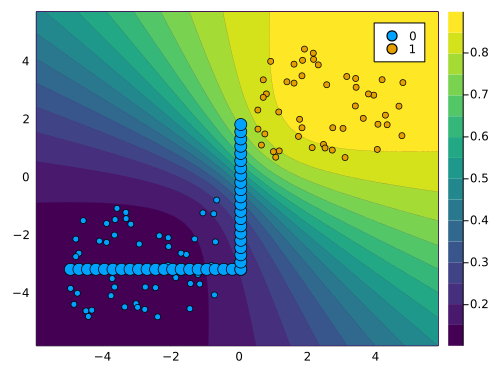
\includegraphics[width=3.33333in,height=2.5in]{www/ce_binary_laplace.png}

}

\caption{\label{fig-binary-laplace}Counterfactual path using greedy
counterfactual generator for Bayesian binary classifier.}

\end{figure}

\hypertarget{custom-models}{%
\subsection{Custom models}\label{custom-models}}

One of our priorities has been to make
\texttt{CounterfactualExplanations} scalable and versatile. In the long
term we aim to add support for more default models and counterfactual
generators. In the short term it is designed to allow users to integrate
models and generators themselves. Ideally, these community efforts will
facilitate our long-term goals. Only two steps are necessary to make any
supervised-learning model compatible with our package\footnote{In order
  for the model to be compatible with the gradient-based default
  generators presented in Section~\ref{sec-start} gradient access is
  also necessary, but any model can also be complemented with a custom
  generator.}:

To demonstrate how this can be done in practice we will now consider
another synthetic example. Once again samples are two-dimensional for
illustration purposes, but this time they are grouped into four
different classes and not linearly separable. To predict class labels
based on features we use a simple deep-learning model trained in
\href{https://fluxml.ai/}{Flux.jl} (\cite{innes2018flux}). The code
below shows the simple model architecture. Note how outputs from the
final layer are note passed through a softmax activation function, since
counterfactual loss is evaluated with respect to logits as we discussed
earlier. The model is trained with dropout for ten training epochs.

\begin{lstlisting}[language = Julia]
n_hidden = 32
output_dim = length(unique(y))
input_dim = 2
model = Chain(
    Dense(input_dim, n_hidden, activation),
    Dropout(0.1),
    Dense(n_hidden, output_dim)
)  
\end{lstlisting}

The code below implements the two steps that are necessary to make the
trained neural network compatible with the package: subtyping and
multiple dispatch. Computing logits amounts to just calling the Flux.jl
model on inputs. Predicted probabilities for labels can than be computed
through softmax.

\begin{lstlisting}[language = Julia]
# Step 1)
struct NeuralNetwork <: Models.FittedModel
    model::Any
end

# Step 2)
# import functions in order to extend
import CounterfactualExplanations.Models: logits
import CounterfactualExplanations.Models: probs 
logits(M::NeuralNetwork, X::AbstractArray) = M.model(X)
probs(M::NeuralNetwork, X::AbstractArray) = softmax(logits(M, X))
M = NeuralNetwork(model)
\end{lstlisting}

Finally, the code below draws a random sample and generates a
counterfactual in a different target class through generic search. The
code very much resembles the earlier examples, with the only notable
difference that for the counterfactual loss function we are now using
the multi-class logit cross-entropy loss. The resulting counterfactual
path is shown in Figure~\ref{fig-multi}. In this case the contour shows
the predicted probability that the input is in the target class
(\(t=4\)). Generic search yields a valid, realistic and unambiguous
counterfactual.

\begin{lstlisting}[language = Julia]
# Randomly selected factual:
using Random
Random.seed!(42)
x_factual = x[rand(1:length(x))]
y_factual = Flux.onecold(
    probs(M, x_factual),unique(y))
target = rand(unique(y)[1:end .!= y_factual]) 
confidence = 0.75

# Counterfactual search:
generator = GenericGenerator(
    0.1,0.1,1e-5,:logitcrossentropy,nothing)
counterfactual = generate_counterfactual(
    generator, x_factual, M, target, confidence)
\end{lstlisting}

\begin{figure}

{\centering 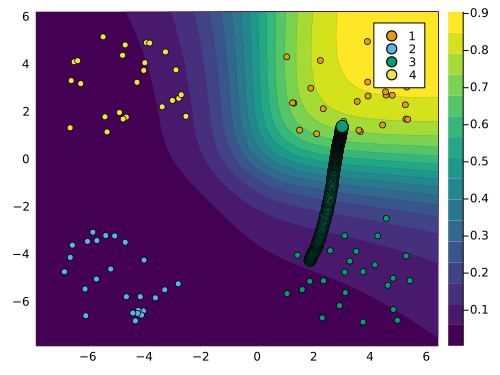
\includegraphics[width=3.33333in,height=2.5in]{www/ce_multi.png}

}

\caption{\label{fig-multi}Counterfactual path using generic
counterfactual generator for multi-class classifier.}

\end{figure}

As before we will also look at the Bayesian setting. Using Laplace
approximation (LA) much in the same way as above we can recover a
Bayesian representation of our neural network in a post-hoc fashion
(\cite{daxberger2021laplace}). Alternatively, we could have considered
using a deep ensemble (\cite{lakshminarayanan2016simple}), Monte Carlo
dropout (\cite{gal2016dropout}) or variational inference. Using the
greedy generator yields the counterfactual path in
Figure~\ref{fig-multi-laplace}. The code that produces these results
follows below.

Contrary to the example involving binary classification above, it is
less clear that counterfactuals for the Bayesian classifier are more
effective in this case. While predictions from this simple Bayesian
neural network are overall more conservative, the model fails to only
produce high-confidence predictions in regions that are abundant with
training samples. This illustrates that the quality of counterfactual
explanations may ultimately depend to some degree on the quality of the
classifier. Put differently, if the quality of the classifier is poor,
we may expect this to come through in the counterfactual explanation.

\begin{lstlisting}
# Fitting the Laplace approximation:
using BayesLaplace
la = laplace(model)
fit!(la, data)

# Model:
# Step 1)
struct LaplaceNeuralNetwork <: Models.FittedModel
    la::BayesLaplace.LaplaceRedux
end

# Step 2)
logits(M::LaplaceNeuralNetwork, X::AbstractArray) = M.la.model(X)
probs(M::LaplaceNeuralNetwork, X::AbstractArray) = BayesLaplace.predict(M.la, X)
M = LaplaceNeuralNetwork(la)

# Counterfactual search:
generator = GreedyGenerator(
    0.25,30,:logitcrossentropy,nothing)
counterfactual = generate_counterfactual(
    generator, x_factual, M, target, confidence) 
\end{lstlisting}

\begin{figure}

{\centering 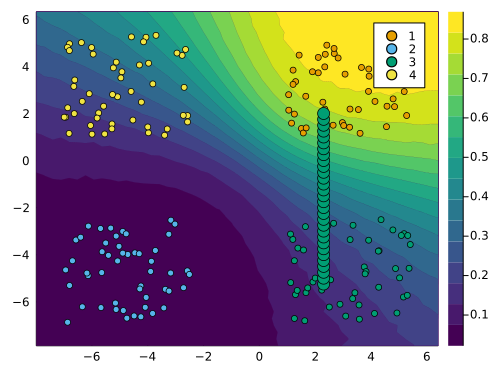
\includegraphics[width=3.33333in,height=2.5in]{www/ce_multi_laplace.png}

}

\caption{\label{fig-multi-laplace}Counterfactual path using generic
counterfactual generator for multi-class classifier with Laplace
approximation.}

\end{figure}

\hypertarget{empirical-example}{%
\subsection{Empirical example}\label{empirical-example}}

Now that we have explained the basic functionality of
\texttt{CounterfactualExplanations} through a few illustrative toy
examples, it is time to consider some real data. The MNIST dataset
contains 60,000 training samples of handwritten digits in the form of
28x28 pixel grey-scale images (\cite{lecun1998mnist}). Each image is
associated with a label indicating the digit (0-9) that the image
represents. The data makes for an interesting case-study of
counterfactual explanations, because humans have a good idea of what
realistic counterfactuals of digits look like. For example, if you were
asked to pick up an eraser and turn the digit in
Figure~\ref{fig-mnist-orig} into a four (4) you would know exactly what
to do: just erase the top part. In \cite{schut2021generating} leverage
this idea to illustrate to the reader that their methodolgy produces
effective counterfactuals. In what follows we replicate some of their
findings. You as the reader are therefore the perfect judge to evaluate
the quality of the counterfactual explanations presented here.

On the model side we will use two pre-trained classifiers\footnote{The
  pre-trained models were stored as package artifacts and loaded through
  helper functions.}: firstly, a simple multi-layer perceptron (MLP)
and, secondly, a deep ensemble composed of five such MLPs following
\cite{schut2021generating}. Deep ensembles are approximate Bayesian
model averages that have been shown to yield high-quality esimtates of
predictve uncertainty for neural networks (\cite{wilson2019case.pdf},
\cite{lakshminarayanan2016simple})). In the previous section we already
created the necessary subtype and methods to make the multi-output MLP
compatible with our package. The code below implements the two necessary
steps for the deep ensemble.

\begin{lstlisting}
using Flux: stack
# Step 1)
struct FittedEnsemble <: Models.FittedModel
    ensemble::AbstractArray
end
# Step 2)
using Statistics
logits(M::FittedEnsemble, X::AbstractArray) = mean(
    stack([m(X) for m in M.ensemble],3), 
    dims=3)
probs(M::FittedEnsemble, X::AbstractArray) = mean(
    stack([softmax(m(X)) for m in M.ensemble],3),
    dims=3)
M_ensemble = FittedEnsemble(ensemble)
\end{lstlisting}

\begin{figure}

{\centering 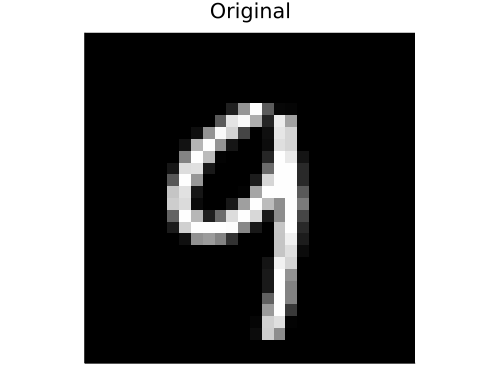
\includegraphics[width=1.66667in,height=1.25in]{www/mnist_original.png}

}

\caption{\label{fig-mnist-orig}A handwritten nine (9) randomly drawn
from the MNIST dataset.}

\end{figure}

For the counterfactual search we will use four different combinations of
classifiers and generators: firstly, the generic approach for the MLP;
secondly, the greedy approach for the MLP; thirdly, the generic approach
for the deep ensemble; and finally, the greedy approach for the deep
ensemble.

\textbf{TBD}

\hypertarget{sec-conclude}{%
\section{Concluding remarks}\label{sec-conclude}}

% **************GENERATED FILE, DO NOT EDIT**************

\bibliographystyle{juliacon}
\bibliography{ref.bib}


\end{document}
